\documentclass{article}

\usepackage[fleqn]{amsmath}
\usepackage{amssymb}
\usepackage{hyperref}
\usepackage{url}
\usepackage{graphicx}
\usepackage{geometry}
\usepackage{babel}
\usepackage{enumitem}
\usepackage{parskip}
\usepackage{chemfig}
\usepackage{pdfpages}
\usepackage{xcolor}
\usepackage{tikz}
\usepackage{fancybox}
\usepackage{makecell}
\usepackage{pgfplots}
\usepackage{soul}
\usepackage{ulem}
\usepackage{wrapfig}
\usepackage{subcaption}
\usepackage[T1]{fontenc}
\usetikzlibrary{decorations.pathreplacing}
\pgfplotsset{compat=1.17}

\geometry{
    a4paper,
    total={170mm, 257mm},
    left=20mm,
    top=20mm
}

\hypersetup{
    colorlinks=true,
    linkcolor=black,
    urlcolor=blue,
    pdftitle={Exam 2023}
}

\newcommand{\figbox}[1]{ 
    \begin{figure*}[ht!]        
        \begin{center}            
            \fbox{#1}        
        \end{center}    
    \end{figure*}
}

% === TEXT ===
\title{\textbf{Maths refreshing course - Exam 2023 \\ HSLU, Semester 1}}
\author{Matteo Frongillo}

\begin{document}

\maketitle

\section*{1a)}
\(x^4 - 24x^2 + 144 = (x^2 - 12)^2\)

\section*{1b)}
\(8t^6 + 27b^3 = 2^3t^{3 \cdot 2} + 3^3 \cdot b^3 = (2x^2)^3 + (3y)^3\) (Unsure of next steps)

\section*{2a, b)}
Unclear

\section*{3a)}
\((t-5)^2(t+k+k^2)\\
    = (t^2 - 10t + 25)(k^2 + k + t)\\
    = t^2k^2+t^2k+t^3-10tk^2-10tk^2-10t^2+25k^2+25k+25t\\
    = t^3+t^2k^2-10tk^2+t^2k-10t^2k-10t^2+25k^2-10tk+25k+25t
\)

\section*{3b)}
\((x+y+2z)^2 = x^2+xy+2xz+yx+y^2+2yz+2zx+4z^2 = x^2+y^2+4z^2+2xy+4xz+4yz\)


\section*{4)}
\(4x^3-4x^2-11x+6=0\)
\[ 2 \hspace{.25cm}
\begin{array}{rrr|r}
    +4 & -4 & -11 & +6 \\
    & +8  & +8  & -6 \\
\hline
    +4 & +4  & -3  & 0
\end{array} \Rightarrow x_1 = 2
\] 
\hspace{2.5cm}$\Downarrow$\\
\phantom{} \hspace{1.3cm}\(4x^2+4x-3=0 \rightarrow x_{2,3}=
    \frac{-4 \mp \sqrt{16+48}}{8}= \frac{-4 \mp 8}{8} \Rightarrow
    x_{2,3} \in \left\{-\frac{3}{2}, \frac{1}{2}\right\}\)

Solution: \(x \in \left\{-\frac{3}{2}, \frac{1}{2}, 2\right\}\)

\section*{5a)}
\(kx^2+(k-1)x+\frac{1}{4}=0 \rightarrow \Delta < 0\)

\(a=k,\ b=k-1,\ c=\frac{1}{4}\)

\(\Rightarrow (k-1)^2-4 \cdot k \cdot \frac{1}{4} = k^2-2k+1-k = k^2-3k+1\)

\(\Rightarrow k^2-3k+1<0 \Rightarrow k_{1,2}=\frac{3 \mp \sqrt{9-4}}{2}\)

\(k_1=\frac{3-\sqrt{5}}{2}; \quad k_2=\frac{3+\sqrt{5}}{2} \Rightarrow
\text{The equation has no real solution in the interval } \frac{3-\sqrt{5}}{2} < k < \frac{3+\sqrt{5}}{2}\)

\section*{5b)}
\(2x^2+x+\frac{1}{4}=0 \rightarrow \Delta=\mp \sqrt{1-2} \rightarrow 
\Delta < 0 \rightarrow x \in \left\{\right\}\)

\section*{6)}
\(2x^2 - 2x +2\)

Simmetry axis: \(x=\frac{-b}{2a}=\frac{2}{4}=\frac{1}{2}\)

Delta (check for intersections with abscissae):
\(b^2 - 4ac = 4-16 = -12 \rightarrow \Delta < 0 \rightarrow\)
No intersection

Vertex: \((V_x, V_y) = \left(\frac{-b}{2a}, f(V_x)\right)=
\left(\frac{1}{2}, \frac{3}{2}\right)\)

Points: \vspace*{-0.5cm}
\begin{center}
    \[\begin{array}{c|c}
        x & y \\
        \hline 0 & 2 \\
        \frac{3}{2} & \frac{7}{2}
    \end{array}\]
\end{center}

Plot:   
\begin{center}
    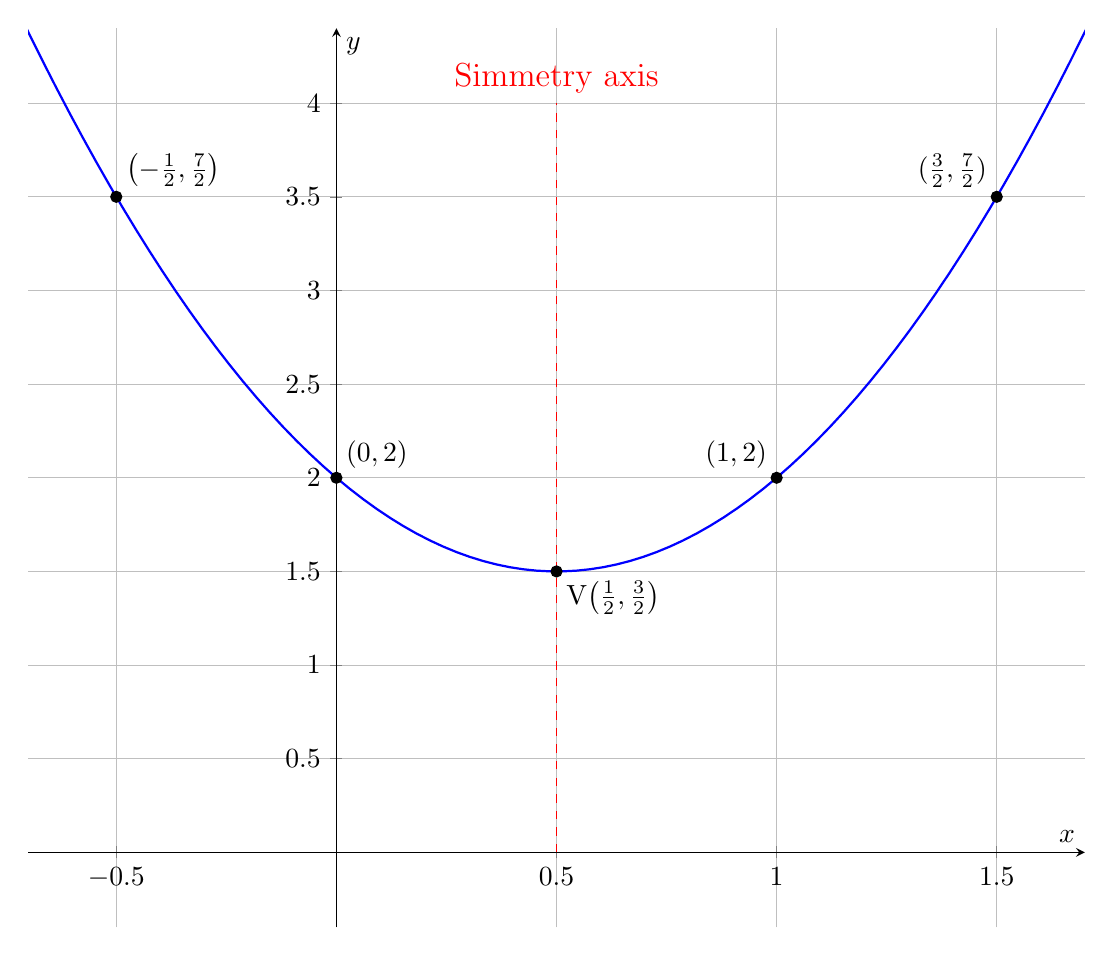
\begin{tikzpicture}
        \begin{axis}[
            axis lines=middle,
            xlabel={$x$},
            ylabel={$y$},
            xmin=-.5, xmax=1.5,
            ymin=0, ymax=4,
            grid=both,
            width=15cm,
            height=13cm,
            enlargelimits,
            samples=100,
            domain=-1:2,
            xtick={-1, -0.5, 0, 0.5, 1, 1.5, 2, 2.5}
        ]
    
        \addplot[blue, thick, domain=-1:2] {2*x^2 - 2*x + 2};
    
        \addplot[mark=*, mark size=2pt] coordinates {(0, 2)} node[above right] {$(0, 2)$};
        \addplot[mark=*, mark size=2pt] coordinates {(1, 2)} node[above left] {$(1, 2)$};
        \addplot[mark=*, mark size=2pt] coordinates {(0.5, 1.5)} node[below right] {V$\left(\frac{1}{2}, \frac{3}{2}\right)$};
        \addplot[mark=*, mark size=2pt] coordinates {(-0.5, 3.5)} node[above right] {$\left(-\frac{1}{2}, \frac{7}{2}\right)$};
        \addplot[mark=*, mark size=2pt] coordinates {(1.5, 3.5)} node[above left] {$(\frac{3}{2}, \frac{7}{2})$};
    
        \draw[dashed, red] (axis cs:0.5,0) -- (axis cs:0.5,4) node[above] {\large Simmetry axis};
    
        \end{axis}
    \end{tikzpicture}  
\end{center}








\end{document}
